\documentclass{article}
\usepackage{graphicx}
\usepackage{url}
\usepackage[utf8]{inputenc}
\usepackage{caption}
\usepackage{subfig}
\captionsetup[table]{name=Tabel }

\title{Hill Climbing vs Simulated Annealing}
\author{Gavrila Maria-Denisa & Virna Stefan-Alexandru}
\date{Octombrie 2022}
\begin{document}
\maketitle
 \begin{abstract}
    Documentul prezinta o analiza ampla asupra algoritmilor de Hill Climbing si Simulated Annealing, punand in prim-plan performantele acestora, precum si particularitatile lor. Vom utiliza variatii ale algoritmului Hill Climbing si impactul functiilor neighbour pentru rezultatele obtinute.
\end{abstract}

\section{Introducere}
Scopul final al temei este atingerea minimului unei functii complexe utilizand variatii ale algoritmului de Hill Climbing si Simulated Annealing. Hill Climbing este o tehnica de optimizare matematica din familia cautarilor locale care gaseste solutii optime pentru problem convexe, iar pentru celelalte functii se opreste doar la optime locale ce nu sunt neaparat cele mai bune din spatiul de cautare. Pentru a observa particularitatile, vom executa o serie de experimente in care vom utiliza functiile DeJong, Schwefel’s, Rastrigin’s, Michaelwicz’s , analizand performantele pentru 5,10,30 de dimensiuni in cazul fiecarei functii. Atat algoritmii de Hill Climbing, cat si cel de Simulated Annealing cauta in maniera euristica solutia optima. In continuare, vom urmari modul de functionare si rezultatele obtinute, precum si diferentele dintre cele 4 variante propuse: Best Improvement Hill Climbing, First Improvement Hill Climbing, Worst Improvement Hill Climbing si Simulated Annealing.

\subsection{Functii}
De Jong's function 1\cite{DeJong}:
$$ f(x) = \sum_{i=1}^n x_i^2,
x_i \in \left[ -5.12, 5.15 \right]$$
Schwefel's function 7\cite{Schwefel}:
$$ f(x) = \sum_{i=1}^n - x_i \cdot sin(\sqrt{|x_i|}),
x_i \in \left[ -500, 500 \right]$$
Rastrigin's function 6\cite{Rastrigin}:
$$ f(x) = A \cdot n + \sum_{i=1}^n \left[ x_i^2 - A \cdot cos(2 \pi x_i) \right],
A = 10, x_i \in \left[ -5.12, 5.15 \right]$$
Michalewicz's function 12\cite{Michalewicz}:
$$ f(x) = -\sum_{i=1}^n sin(x_i) \cdot(sin(\frac{i \cdot x_i^2}{\pi}))^{2 \cdot m},
i=1:n, m=10, 0 \le x_i \le \pi$$
\section{Metode}

\subsection{Hill Climbing}
Hill Climbing este o tehnica care porneste de la o solutie aleatoare si va incerca sa gaseasca optimul prin imbunatatiri successive. In cazul in care functia nu este convexa, exista riscul blocarii in minime locale, moment in care se poate reporni algortmul dintr-un nou punct aleator. O imbunatatire pentru aceasta problema este agloritmul de Simulated Annealing.\\
\\
Pasi de executie:

Fie S $\in \omega$ \footnote{$\omega$ = spatiul de cautare}, o solutie generata aleator

Cat timp nu am gasit rezultatul si k \footnote{k = pasul curent} $ < k_{max}$ 

\hspace*{10mm} Alegem n $\in$ neighbours\footnote{neighbours(S) = multimea vecinilor lui S}(S)

\hspace*{10mm} Daca $f(n) < f(S) => S = n$\\\\

O particularitate a implementarii utilizate este reprezentarea solutiei sub forma binara, mai exact un vector de lungime $d*\lceil log_2((b-a) * 10^p) \rceil$, unde d este dimensiunea functiei, a si b sunt capetele de interval, iar p este precizia utilizata in reprezentarea numerica.\\\\
In cadrul procedurii de initializare vom construi aleator o solutie de pornire S $\in \omega$, spatiul de cautare.\\\\
Functia neighbors(s) difera in functie de variatia algoritmului Hill Climbing. La baza, toate folosesc o notiune de vecinatate comuna. In acest context, consideram vecin orice reprezentare binara ce difera de S printr-un singur bit.\\\\
Cautarea se opreste atunci cand k, contorul iteratiei curente, ajunge la valoarea $k_{max}$ sau cand evaluarea solutiei $f(S) < \epsilon$. Valoarea acestui $\epsilon$ este determinat de minimul functiei pentru care vom executa experimentul.

\subsubsection{First Improvement}
Vom alege primul vecin cu o solutie imbunatatita fata de cea originala.
\subsubsection{Best Improvement}
Dintre vecinii generati il vom alege pe cel cu cel mai bun improvement.
\subsubsection{Worst Improvement}
Vom alege vecinul cu imbunatatirea cea mai slaba.
\subsection{Simulated Annealing}
Simulated Annealing este un algoritm capabil sa scape din optimele locale. Este o tehnica populara datorita usurintei de implementare, proprietatilor de convergenta si utilizarea Hill Climbing pentru evadarea din minime locale. 
Numele provine de la analogia cu procesul de incalzire, urmat de racire lenta pentru a favoriza solidificarea uniforma, fara defecte. Daca procesul de racire este suficient de lent, atunci produsul va avea o integritate structurala superioara. Algoritmul simuleaza acest comportament termodinamic in cautarea minumului global. Sa adopta o miscare iterativa in functie de variatia temperaturii pentru a imita acest proces. Pornim de la o temperatura de start arbitrar aleasa. Numarul de vecini verificati la fiecare pas este proportional cu temperatura. Dintre acestia, alegem solutia mai buna, insa exista probabilitatea alegerii unei solutii mai slabe (bazata pe formula ~ T), in speranta ca vecinii acestei noi solutii ar putea duce totusi la un rezultat mai bun. Totodata generarea vecinilor este influentata de temperatura, aceasta nefiind limitata la editarea unui singur bit, spre deosebire de implementarea folosita in cadrul Hill Climbingului.\\\\
Fie S $\in \omega$, o solutie generata aleator\\
$T = T_{initial}$\\
Cat timp $f(S) \ge \epsilon$ sau $k < k_{max}$:\\
\hspace*{10mm} $M_k = MT_k(T)$\footnote{$MT_k(T)$ = functia ce returneaza numarul de vecini verificati la temperatura T;} \\
\hspace*{10mm} Pentru $i = 0, i < M_k$:\\
\hspace*{10mm}\hspace*{10mm} Fie $S' \in neighbours(S, T)$\footnote{neighbours(S,T) = vecinii lui S, in functie de temperatura T;} \\
\hspace*{10mm}\hspace*{10mm} Daca $f(S') < f(S)$\footnote{f(S) = functia de optimizat}$ => S = S'$\\
\hspace*{10mm}\hspace*{10mm} Altfel, S = S', cu probabilitatea $exp(\frac{-|f(S’)-f(S)|)}{T})$\\
\hspace*{10mm} T = q(T)\footnote{q(T) = functia de racire}\\\\
Reprezentarea solutiei se face in acelasi mod sugerat la algoritmul de Hill Climbing, insa pentru generarea vecinilor propunem o varianta influentata de temperatura, ce ofera rezultate mai bune comparative cu schimbarea aleatorie a unui singur bit (in special in testele pe probleme cu dimensionalitate crescuta). Astfel, numarul de biti ce pot fi modificati in mod aleatoriu  sunt proportionali cu numarul de dimensiuni ale problemei si temperatura curenta. In executie putem observa ca la inceput (T este mare), algoritmul exploreaza un numar mai mare de vecini (conform valorii lui $MT_k(T)$), si mai variati ($neighbours(S,T)$), urmand ca, impreuna cu scaderea T, numarul de vecini verificati sa scada, impreuna cu variatia acestora.
\section{Descrierea experimentelor}
Am rulat algoritmii pe cele 4 functii prezentate mai sus, DeJong, Schwefel’s, Rastrigin’s, Michaelwicz’s, cu cele 3 variante de dimensionalitate, $d \in \{5, 10, 30\}$. fiecare experiment a fost rulat de 40 de ori, pentru a obtine o viziune de ansamblu cat mai corecta asupra performantei fiecarui algoritm. In experimente, am utilizat $k_{max} = 5000$ si am observat ca aceasta valoare este suficent de mare pentru a produce rezultate satisfacatoare in cele mai multe cazuri. In ceea ce priveste precizia, aceasta a fost de 5 zecimale. experimentele au fost rulate cu o implementare in C++17 a algoritmilor descrisi, pe un sistem Ubuntu 20.04.5. Pentru a reduce considerabil timpul de executie am implementat o functionalitate de "kill on plateau", care opreste fortat un experiment Hill Climbing daca evaluarea nu se modifica timp de 150 de executii succesive. In cadrul Simulated Annealing am folosit $T_{initial}$ = 100, si $q(T) = T \cdot 0.99$
\section{Rezultate experimentale} 
In urma rularii experimentelor am colectat urmatoarele rezultate. In sectiunea de mai jos se poate observa progresul algoritmilor de cautare a minimului functiilor, in raport cu iteratia curenta, precum si rezultatele fiecarei rulari. \\
Au fost executate 40 de rulari pentru fiecare permutare (functie - algoritm - dimensionalitate), exceptand Rastring - Simulated Annealing - 30 de dimensiuni, unde  au fost executate doar 30 de iteratii. \\
Numarul redus de iteratii este dat de conditia de early stopping bazata pe $\epsilon$, dar si de oprirea algoritmului in cazul in care acesta nu gaseste o solutie diferita (valabil doar pentru Hill Climbing).
\clearpage
\begin{figure}
    \centering
    \subfloat[\centering deJong - Best Improvement]{{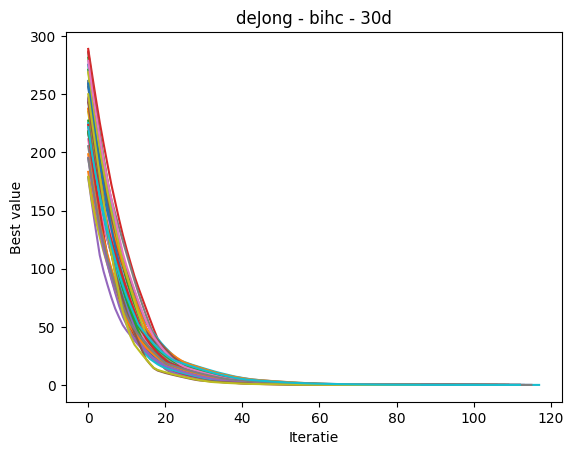
\includegraphics[width=5cm]{bihc_dejong_30.png} }}%
    \qquad
    \subfloat[\centering deJong - First Improvement]{{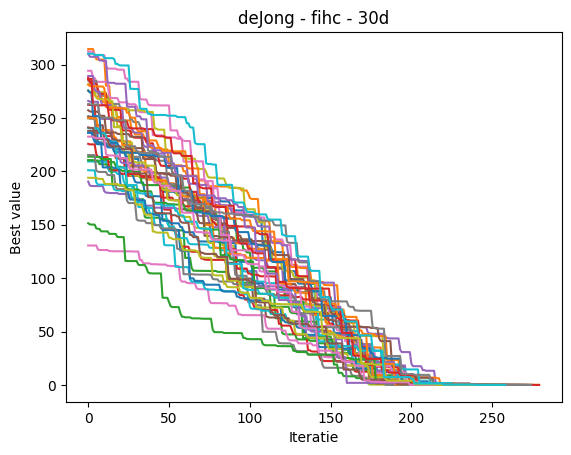
\includegraphics[width=5cm]{fihc_dejong_30.png} }}%
    \centering
    \subfloat[\centering michalewicz - Best Improvement]{{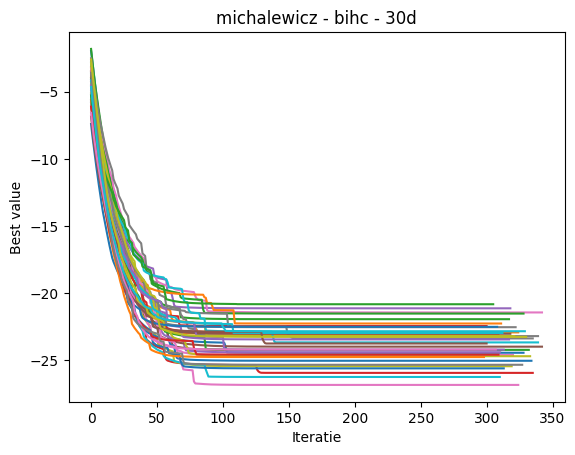
\includegraphics[width=5cm]{bihc_michalewicz_30.png} }}%
    \qquad
    \subfloat[\centering michalewicz - First Improvement]{{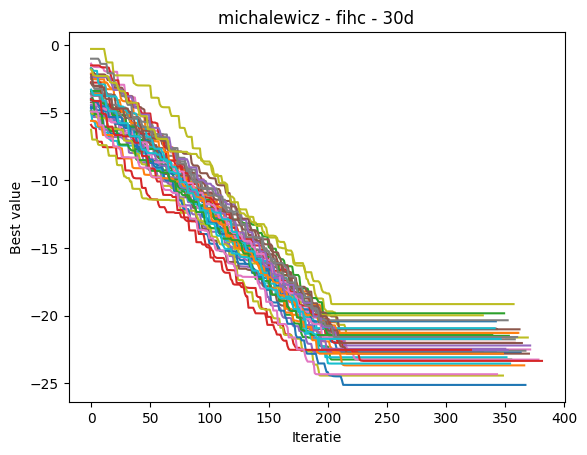
\includegraphics[width=5cm]{fihc_michalewicz_30.png} }}%
    \centering
    \subfloat[\centering schwefel - Best Improvement]{{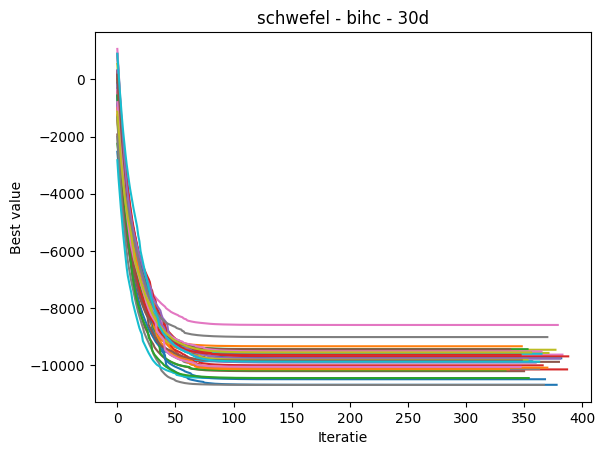
\includegraphics[width=5cm]{bihc_schwefel_30.png} }}%
    \qquad
    \subfloat[\centering schwefel - First Improvement]{{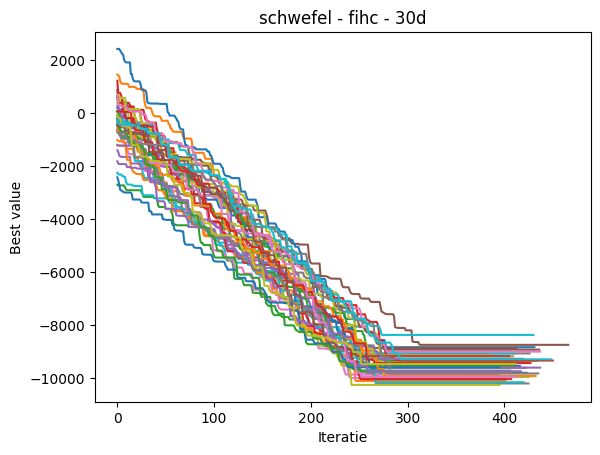
\includegraphics[width=5cm]{fihc_schwefel_30.png} }}%
    \caption{Evolutia minimului in functie de numarul de iteratii}%
    \label{tab:example}
\end{figure}
\clearpage
\subsection{Best Improvement Hill Climbing}
\begin{table}[h]
\begin{tabular}{ccccccccc}
\hline
Functie&D&Min&Max&Avg&Std&Mean&Q1&Q3\\
\hline
\hline
deJong&5&0.0031&0.00967&0.00754&0.0015&0.00754&0.00675&0.00871 \\ \hline
deJong&10&0.0071&0.00998&0.00881&0.00081&0.00881&0.00825&0.00952 \\ \hline
deJong&30&0.00905&0.00997&0.0096&0.00027&0.0096&0.00941&0.00983 \\ \hline
\hline
schwefel&5&-1976.16&-1142.96&-1636.1385&213.49224&-1636.1385&-1824.62&-1503.295 \\ \hline
schwefel&10&-3824.77&-2497.02&-3290.29575&288.24926&-3290.29575&-3473.8375&-3079.9875 \\ \hline
schwefel&30&-10686.8&-8589.48&-9823.833&417.32899&-9823.833&-10095.375&-9553.8375 \\ \hline
\hline
michalewicz&5&-4.6094&-2.92622&-3.83783&0.49337&-3.83783&-4.21466&-3.50423 \\ \hline
michalewicz&10&-9.0125&-5.95644&-7.65102&0.763&-7.65102&-8.21891&-7.23091 \\ \hline
michalewicz&30&-26.817&-20.8159&-23.66052&1.38422&-23.66052&-24.5724&-22.88192 \\ \hline
\hline
rastringin&5&2.23078&18.4765&9.73974&3.57531&9.73974&7.56813&12.13152 \\ \hline
rastringin&10&8.15926&36.0616&20.49974&7.58287&20.49974&14.78742&25.63278 \\ \hline
rastringin&30&41.2225&85.7363&63.63507&10.09825&63.63507&56.53042&70.0331 \\ \hline
\hline
\end{tabular}
\caption{Rezultate Best Improvement Hill Climbing} \footnotesize{D = numarul de dimensiuni}; {Min = valoarea minima}; {Max = valoarea maxima}; {Avg = media valorilor}; {Std = deviatia standard}; {Mean = mediana};
\end{table}

\subsubsection{DeJong}
\begin{tabular}{cccccc}
\hline
ultima iteratie 5D& optim&ultima iteratie 10D& optim&ultima iteratie 30&optim\\
\hline
9&0.00741055&37&0.00945665&98&0.0097818 \\ \hline
13&0.00873875&36&0.00995516&105&0.00955233 \\ \hline
10&0.00740351&25&0.00824943&110&0.00954661 \\ \hline
14&0.00672896&30&0.00963109&113&0.00991742 \\ \hline
10&0.00945906&26&0.0097432&99&0.00904748 \\ \hline
14&0.0081993&42&0.00952353&95&0.00983263 \\ \hline
12&0.00747393&32&0.00853148&116&0.00924658 \\ \hline
20&0.00941347&33&0.00855225&113&0.0093391 \\ \hline
15&0.00507305&37&0.00813293&101&0.0092121 \\ \hline
14&0.00310352&23&0.00883615&109&0.0096454 \\ \hline
20&0.00715597&28&0.00824294&114&0.00919527 \\ \hline
12&0.00870511&32&0.00899718&109&0.00917949 \\ \hline
14&0.00849124&28&0.00966091&98&0.00980379 \\ \hline
13&0.00807148&29&0.00877622&113&0.00970863 \\ \hline
13&0.00676342&31&0.00787445&103&0.00987692 \\ \hline
12&0.00810789&25&0.00941074&105&0.00994366 \\ \hline
10&0.00949253&34&0.00727477&104&0.00984468 \\ \hline
16&0.00723725&29&0.00891725&93&0.00941515 \\ \hline
12&0.00502516&32&0.00997914&97&0.00972564 \\ \hline
17&0.00967497&24&0.00888079&118&0.00974108 \\ \hline
18&0.00661454&29&0.00710258&104&0.00916784 \\ \hline
12&0.00630787&31&0.00961702&106&0.00955483 \\ \hline
18&0.00759328&32&0.00817876&97&0.00987057 \\ \hline
18&0.00806884&30&0.00773066&88&0.00967243 \\ \hline
11&0.00883378&25&0.00931274&93&0.00996626 \\ \hline
16&0.00861964&35&0.00828347&107&0.00967472 \\ \hline
21&0.00819812&28&0.00996993&107&0.00983989 \\ \hline
15&0.003684&29&0.00886312&116&0.00925836 \\ \hline
15&0.00788467&28&0.00952086&103&0.00962401 \\ \hline
14&0.00628274&39&0.00726713&104&0.00951178 \\ \hline
15&0.00631891&33&0.0094051&102&0.00939227 \\ \hline
13&0.00928155&36&0.0072487&98&0.00990229 \\ \hline
14&0.00758431&36&0.00931725&107&0.00973772 \\ \hline
18&0.00882269&31&0.00959758&110&0.00960172 \\ \hline
14&0.00675669&27&0.00851542&100&0.00904605 \\ \hline
12&0.0072586&30&0.00811873&96&0.0098776 \\ \hline
13&0.00634586&28&0.00845411&107&0.00972807 \\ \hline
14&0.00723907&26&0.00913955&110&0.00942123 \\ \hline
11&0.00915484&23&0.00971933&87&0.00968381 \\ \hline
15&0.00921411&28&0.00847909&113&0.00994111 \\ \hline
\end{tabular}
\subsubsection{Schwefel’s}
\begin{tabular}{cccccc}
\hline
ultima iteratie 5D& optim&ultima iteratie 10D& optim&ultima iteratie 30&optim\\
\hline
191&-1622.15&225&-2979.85&343&-9873.38 \\ \hline
191&-1942.03&227&-2889.18&349&-9335.01 \\ \hline
186&-1508.04&235&-3076.38&359&-9528.32 \\ \hline
194&-1508.04&229&-3559.95&367&-10002.0 \\ \hline
182&-1857.83&242&-3824.77&358&-9856.27 \\ \hline
187&-1372.79&233&-3618.48&351&-10206.3 \\ \hline
201&-1142.96&227&-3081.19&384&-9626.9 \\ \hline
198&-1503.71&236&-3384.21&364&-9555.15 \\ \hline
187&-1626.48&230&-3288.77&378&-9456.66 \\ \hline
199&-1821.97&241&-2952.46&357&-9863.81 \\ \hline
188&-1707.69&227&-3318.08&379&-10683.1 \\ \hline
204&-1361.24&236&-2497.02&346&-9502.88 \\ \hline
197&-1499.79&231&-3259.03&354&-9436.32 \\ \hline
184&-1623.66&227&-3115.33&388&-10144.4 \\ \hline
204&-1695.29&222&-3764.11&351&-9792.56 \\ \hline
191&-1699.72&223&-3481.0&381&-9879.87 \\ \hline
183&-1503.32&235&-3118.64&380&-8589.48 \\ \hline
196&-1368.77&223&-3471.45&364&-10133.1 \\ \hline
188&-1684.74&228&-3433.57&372&-9568.14 \\ \hline
180&-1929.56&223&-3537.81&366&-9597.41 \\ \hline
191&-1860.44&229&-2958.4&383&-9753.93 \\ \hline
186&-1725.5&235&-3267.73&371&-10082.8 \\ \hline
197&-1832.57&211&-3464.98&335&-10176.8 \\ \hline
199&-1577.05&231&-3549.3&389&-9687.77 \\ \hline
188&-1503.22&224&-3187.76&382&-9766.35 \\ \hline
186&-1389.59&229&-3072.03&339&-9440.85 \\ \hline
195&-1346.63&216&-3312.41&366&-9512.81 \\ \hline
178&-1976.16&231&-3200.23&368&-10686.8 \\ \hline
203&-1553.78&237&-2702.48&354&-9810.38 \\ \hline
180&-1963.79&233&-2994.45&345&-10462.6 \\ \hline
190&-1788.97&217&-3211.78&369&-10488.2 \\ \hline
194&-1895.32&219&-3057.94&338&-10138.9 \\ \hline
180&-1620.08&220&-3699.36&355&-10447.2 \\ \hline
200&-1792.17&220&-3276.77&348&-9632.15 \\ \hline
180&-1857.44&230&-3350.02&361&-9905.4 \\ \hline
189&-1673.25&232&-3452.41&349&-9836.11 \\ \hline
194&-1583.41&222&-3713.27&348&-10057.0 \\ \hline
193&-1151.31&219&-3450.07&371&-9012.85 \\ \hline
185&-1467.18&223&-3671.17&357&-9549.9 \\ \hline
188&-1907.9&236&-3367.99&364&-9873.46 \\ \hline
\end{tabular}
\subsubsection{Rastrigin’s}
\begin{tabular}{cccccc}
\hline
ultima iteratie 5D& optim&ultima iteratie 10D& optim&ultima iteratie 30&optim\\
\hline
184&17.001&221&8.15926&335&62.1094 \\ \hline
183&9.62585&216&8.46159&333&51.3102 \\ \hline
182&7.21063&216&12.2208&331&68.6952 \\ \hline
182&7.1542&214&19.2369&346&57.0416 \\ \hline
193&8.63089&224&20.647&337&68.9271 \\ \hline
185&12.1542&227&30.0668&335&69.9869 \\ \hline
183&12.3699&216&14.3648&338&45.9088 \\ \hline
185&8.15421&207&31.451&324&49.1658 \\ \hline
184&4.46662&220&14.8668&328&62.8648 \\ \hline
177&6.96471&229&12.1492&356&63.3187 \\ \hline
187&2.23078&220&27.6121&345&54.9969 \\ \hline
185&13.9033&208&31.8227&344&54.2475 \\ \hline
188&8.90325&205&19.0987&357&67.9045 \\ \hline
181&18.4765&220&16.3497&343&62.6989 \\ \hline
180&10.2106&218&32.376&345&83.4286 \\ \hline
181&2.23078&221&26.2681&332&71.8696 \\ \hline
184&12.3185&208&8.68226&332&69.2497 \\ \hline
190&12.1391&222&20.5704&327&68.8285 \\ \hline
183&6.96976&225&19.7649&330&51.0176 \\ \hline
184&8.21064&215&20.0373&324&65.7368 \\ \hline
192&9.38498&212&25.421&342&71.6334 \\ \hline
186&12.1593&211&20.519&336&65.7781 \\ \hline
181&16.4709&223&14.5493&357&64.1006 \\ \hline
179&7.6873&213&10.6208&350&58.8383 \\ \hline
180&11.1593&215&36.0616&358&49.4382 \\ \hline
184&3.23585&218&35.9907&341&82.0802 \\ \hline
179&11.8368&227&22.1089&325&52.511 \\ \hline
181&12.129&210&15.4061&321&71.64 \\ \hline
182&11.8368&219&16.4011&335&70.1717 \\ \hline
190&11.1593&206&13.3749&361&70.9043 \\ \hline
193&6.15924&207&30.4374&350&60.6753 \\ \hline
183&9.62585&213&18.7602&328&58.3367 \\ \hline
179&12.1542&218&21.6256&328&41.2225 \\ \hline
185&7.97986&214&18.775&326&66.3065 \\ \hline
184&9.97483&215&13.6621&340&69.5137 \\ \hline
183&8.90831&213&33.5137&371&85.7363 \\ \hline
182&11.8368&219&20.77&336&48.5712 \\ \hline
181&9.9184&220&18.8617&340&62.8496 \\ \hline
180&11.1905&217&17.6108&344&70.227 \\ \hline
178&5.45653&222&21.3135&358&75.5613 \\ \hline
\end{tabular}
\subsubsection{Michaelwicz’s}
\begin{tabular}{cccccc}
\hline
ultima iteratie 5D& optim&ultima iteratie 10D& optim&ultima iteratie 30&optim\\
\hline
181&-3.91901&211&-7.52875&329&-24.4255 \\ \hline
178&-4.49514&204&-7.7156&310&-23.0269 \\ \hline
178&-2.92622&220&-7.28144&318&-21.9279 \\ \hline
178&-4.16151&213&-8.40654&336&-25.9214 \\ \hline
181&-4.48895&220&-7.15179&319&-21.1188 \\ \hline
195&-2.98061&216&-8.21477&312&-24.2235 \\ \hline
182&-3.71147&209&-6.69316&343&-21.426 \\ \hline
181&-3.01791&205&-7.60174&340&-23.1854 \\ \hline
177&-3.23221&215&-7.99394&320&-25.4274 \\ \hline
182&-3.96093&216&-8.38886&311&-26.2258 \\ \hline
189&-3.54911&210&-8.2677&335&-25.0212 \\ \hline
175&-4.49528&237&-6.34907&325&-22.9107 \\ \hline
185&-4.0395&218&-5.95644&329&-21.5098 \\ \hline
187&-3.74104&213&-7.78239&301&-22.4348 \\ \hline
186&-4.22092&206&-7.07897&311&-24.391 \\ \hline
181&-2.95064&217&-7.9956&343&-23.9715 \\ \hline
190&-3.16161&212&-6.4108&325&-26.817 \\ \hline
180&-4.43745&214&-7.93226&336&-23.359 \\ \hline
181&-3.90044&214&-8.51057&322&-23.1849 \\ \hline
181&-4.4524&227&-6.26587&340&-23.6549 \\ \hline
187&-3.76895&221&-8.09958&314&-25.5861 \\ \hline
185&-3.26428&211&-5.97597&312&-22.2482 \\ \hline
189&-4.36977&220&-8.23133&333&-24.2091 \\ \hline
181&-3.53663&199&-8.89748&299&-22.9012 \\ \hline
183&-3.96863&211&-7.74507&318&-23.4319 \\ \hline
185&-3.77944&206&-7.74161&319&-23.0107 \\ \hline
180&-3.56101&210&-7.38238&321&-24.5919 \\ \hline
10&-4.6094&211&-7.1911&323&-22.5224 \\ \hline
190&-3.26695&207&-7.24418&334&-24.6818 \\ \hline
181&-3.74631&211&-7.79846&313&-22.9514 \\ \hline
183&-4.01962&211&-8.59074&309&-22.497 \\ \hline
182&-4.16986&211&-7.58716&299&-24.7433 \\ \hline
187&-3.27752&221&-9.0125&306&-20.8159 \\ \hline
185&-4.21258&217&-7.47224&310&-24.5659 \\ \hline
181&-4.19772&226&-8.17173&314&-24.1957 \\ \hline
185&-3.40702&208&-8.56855&301&-23.7356 \\ \hline
179&-4.45023&217&-7.48755&308&-24.183 \\ \hline
189&-4.47331&218&-6.8604&328&-25.3191 \\ \hline
182&-3.74102&212&-8.4902&331&-23.243 \\ \hline
185&-3.85077&205&-7.9664&330&-22.8241 \\ \hline
\end{tabular}


\subsection{First Improvement Hill Climbing}
\begin{table}[h]
\begin{tabular}{ccccccccc}
\hline
Functie&D&Min&Max&Avg&Std&Mean&Q1&Q3\\
\hline
\hline
deJong&5&7e-05&0.00933&0.00379&0.00263&0.00379&0.00128&0.0054 \\ \hline
deJong&10&0.0&0.00921&0.00367&0.00281&0.00367&0.00112&0.00518 \\ \hline
deJong&30&0.00011&0.00902&0.00284&0.0025&0.00284&0.001&0.00382 \\ \hline
\hline
schwefel&5&-1941.92&-1227.17&-1537.06&172.0996&-1537.06&-1617.4275&-1454.26 \\ \hline
schwefel&10&-3871.0&-2504.57&-3123.5345&271.11565&-3123.5345&-3325.1775&-2986.6025 \\ \hline
schwefel&30&-10266.0&-8379.34&-9522.6035&443.35171&-9522.6035&-9886.5825&-9186.51 \\ \hline
\hline
michalewicz&5&-4.65392&-1.522&-3.47995&0.65029&-3.47995&-3.83833&-3.14386 \\ \hline
michalewicz&10&-8.5915&-5.30489&-7.15793&0.87425&-7.15793&-7.7947&-6.44126 \\ \hline
michalewicz&30&-25.1299&-19.1537&-22.10534&1.27305&-22.10534&-22.81755&-21.2869 \\ \hline
\hline
rastringin&5&4.2207&29.9895&12.22156&4.95122&12.22156&9.56563&13.79415 \\ \hline
rastringin&10&10.2006&48.1547&24.65029&9.88588&24.65029&17.333&30.89888 \\ \hline
rastringin&30&47.4789&103.256&74.04023&15.01948&74.04023&64.21623&86.21738 \\ \hline
\hline
\end{tabular}
\caption{Rezultate First Improvement Hill Climbing} \footnotesize{D = numarul de dimensiuni}; {Min = valoarea minima}; {Max = valoarea maxima}; {Avg = media valorilor}; {Std = deviatia standard}; {Mean = mediana};
\end{table}


\subsubsection{DeJong}
\begin{tabular}{cccccc}
\hline
ultima iteratie 5D& optim&ultima iteratie 10D& optim&ultima iteratie 30&optim\\
\hline
39&0.00278041&77&0.00105153&213&0.00886919 \\ \hline
34&0.00227812&73&0.00921444&207&0.00420109 \\ \hline
39&7.02881e-05&75&6.91732e-05&231&0.00135511 \\ \hline
41&0.00513169&87&0.00186273&259&0.000680126 \\ \hline
36&0.00567272&78&0.00812026&273&0.00142574 \\ \hline
43&0.000151286&71&0.00377374&256&0.00144646 \\ \hline
33&0.000937598&78&0.00850846&268&0.00113282 \\ \hline
28&0.00306561&55&0.00706916&259&0.000247669 \\ \hline
41&0.00449647&79&0.00209281&249&0.00822444 \\ \hline
36&0.00270573&69&0.00152933&267&0.00719104 \\ \hline
36&0.00345674&65&0.000616024&257&0.00543694 \\ \hline
41&0.000480442&69&0.00678568&280&0.000509116 \\ \hline
42&0.00383034&86&1.08361e-06&220&0.00117069 \\ \hline
32&0.00612875&83&0.00222436&260&0.000113624 \\ \hline
45&0.00884135&84&0.00302021&242&0.000677239 \\ \hline
23&0.00932605&76&0.00324534&276&0.0059376 \\ \hline
42&0.00179755&85&8.44409e-06&211&0.00901713 \\ \hline
38&0.00257825&80&0.00677328&245&0.00200186 \\ \hline
40&0.00531235&89&0.00277218&251&0.000847192 \\ \hline
39&0.00511631&75&0.00129752&251&0.00282281 \\ \hline
40&0.00111057&93&0.00488294&249&0.00116525 \\ \hline
30&0.000811197&83&0.000252923&264&0.00213592 \\ \hline
33&0.000868352&66&0.00464312&249&0.00130382 \\ \hline
37&0.000944787&98&0.00485024&246&0.00335078 \\ \hline
34&0.00587455&71&0.00813082&258&0.00252596 \\ \hline
45&0.001883&60&0.00853026&269&0.00369022 \\ \hline
27&0.00858225&75&0.00429329&255&0.00285297 \\ \hline
36&0.00823505&77&0.00503296&257&0.00518359 \\ \hline
33&0.00529529&90&0.000483015&275&0.00570218 \\ \hline
45&0.000842079&89&0.000209036&227&0.00105412 \\ \hline
42&0.00314487&72&0.00463371&272&0.0063727 \\ \hline
39&0.00075223&70&0.000533675&235&0.00267846 \\ \hline
34&0.00677355&69&0.00772393&205&0.00084528 \\ \hline
32&0.00482311&77&0.00139493&280&0.000477451 \\ \hline
33&0.00756342&75&0.004582&234&0.000124741 \\ \hline
45&0.0036135&87&0.00114005&247&0.00140957 \\ \hline
36&0.00133432&77&0.00405972&243&0.00369735 \\ \hline
40&0.00336208&79&0.0010477&275&0.00367955 \\ \hline
39&0.00439619&82&0.00563014&257&0.00178847 \\ \hline
33&0.00738784&82&0.00483121&259&0.000400611 \\ \hline
\end{tabular}
\subsubsection{Schwefel’s}
\begin{tabular}{cccccc}
\hline
ultima iteratie 5D& optim&ultima iteratie 10D& optim&ultima iteratie 30&optim\\
\hline
207&-1475.94&255&-3068.39&432&-8842.73 \\ \hline
195&-1461.33&250&-2866.55&402&-10115.0 \\ \hline
209&-1358.08&251&-2993.25&426&-9952.34 \\ \hline
188&-1476.04&256&-3078.98&411&-9597.3 \\ \hline
207&-1465.97&240&-3325.03&423&-9621.53 \\ \hline
196&-1929.45&250&-2935.24&414&-8873.23 \\ \hline
192&-1826.92&249&-3443.23&396&-9875.55 \\ \hline
201&-1388.63&254&-3070.32&427&-9076.68 \\ \hline
195&-1584.31&249&-3069.81&435&-9361.22 \\ \hline
209&-1607.06&251&-2504.57&412&-9082.31 \\ \hline
198&-1262.43&246&-3111.62&417&-9546.14 \\ \hline
206&-1578.87&265&-3084.61&410&-9188.59 \\ \hline
203&-1538.59&249&-3010.05&422&-9341.17 \\ \hline
192&-1704.77&238&-3421.81&451&-9345.58 \\ \hline
202&-1346.63&247&-2801.01&420&-9280.47 \\ \hline
193&-1504.84&268&-2821.98&467&-8754.04 \\ \hline
196&-1484.6&235&-3159.74&402&-10007.7 \\ \hline
203&-1615.51&260&-3517.47&426&-10210.9 \\ \hline
198&-1463.46&248&-3147.28&396&-10266.0 \\ \hline
196&-1588.56&248&-3009.39&421&-10163.6 \\ \hline
201&-1258.68&235&-3358.75&424&-9807.97 \\ \hline
193&-1623.18&236&-3227.72&388&-9146.78 \\ \hline
200&-1446.04&257&-2593.91&410&-9550.47 \\ \hline
188&-1860.65&250&-3191.06&408&-10047.3 \\ \hline
193&-1581.39&236&-3871.0&438&-9612.55 \\ \hline
210&-1333.84&252&-3035.49&437&-8934.93 \\ \hline
191&-1681.19&228&-3325.62&438&-9009.28 \\ \hline
206&-1792.07&262&-2826.0&409&-9789.8 \\ \hline
203&-1467.69&233&-3337.0&433&-9938.83 \\ \hline
206&-1457.0&253&-3400.75&431&-8379.34 \\ \hline
199&-1692.78&246&-3296.26&396&-9598.93 \\ \hline
193&-1227.17&253&-2540.91&433&-9919.68 \\ \hline
194&-1707.28&247&-3132.87&407&-9727.91 \\ \hline
209&-1487.77&256&-3129.26&428&-9441.31 \\ \hline
196&-1941.92&238&-3346.07&418&-9750.06 \\ \hline
197&-1486.9&263&-3240.07&406&-9180.27 \\ \hline
193&-1490.14&241&-3212.11&413&-9957.17 \\ \hline
205&-1446.04&248&-3515.19&436&-9833.36 \\ \hline
204&-1338.07&244&-2966.66&413&-9476.76 \\ \hline
189&-1500.61&240&-2954.35&449&-9299.36 \\ \hline
\end{tabular}
\subsubsection{Rastrigin’s}
\begin{tabular}{cccccc}
\hline
ultima iteratie 5D& optim&ultima iteratie 10D& optim&ultima iteratie 30&optim\\
\hline
190&8.95463&229&10.2006&376&67.6488 \\ \hline
185&9.97483&232&22.1905&379&88.7215 \\ \hline
187&11.1391&220&34.3989&371&54.0155 \\ \hline
191&10.2157&220&10.3799&355&103.02 \\ \hline
188&12.3901&248&13.8664&395&64.0438 \\ \hline
190&11.1542&220&15.868&353&71.0881 \\ \hline
189&18.159&223&28.3076&371&92.0662 \\ \hline
192&10.4717&211&47.7345&366&47.4789 \\ \hline
197&8.63089&228&12.3897&375&82.8027 \\ \hline
178&9.94958&219&16.4213&358&85.6934 \\ \hline
183&10.1904&223&28.0938&360&50.3817 \\ \hline
190&9.62585&220&21.3295&365&81.6911 \\ \hline
195&21.8065&235&18.8466&374&71.4415 \\ \hline
186&18.4765&217&12.1489&366&77.2785 \\ \hline
188&8.68731&218&13.8516&383&82.5821 \\ \hline
179&12.9033&242&34.4312&345&59.4382 \\ \hline
189&10.4717&234&31.0938&353&89.0134 \\ \hline
189&10.2106&232&15.9333&368&69.3907 \\ \hline
191&29.9895&226&24.3961&365&68.6845 \\ \hline
189&14.1189&218&25.3245&347&90.9522 \\ \hline
188&12.9748&228&19.3951&371&62.2919 \\ \hline
190&5.995&237&30.5342&399&87.9785 \\ \hline
186&14.2356&227&18.159&341&97.1563 \\ \hline
195&9.38498&228&30.8339&377&68.7406 \\ \hline
184&13.2157&221&48.1547&389&73.8606 \\ \hline
185&12.3699&210&42.1375&374&47.5536 \\ \hline
190&9.21568&223&20.4263&379&80.4089 \\ \hline
188&4.70243&213&17.6369&349&103.256 \\ \hline
181&21.1952&223&35.3344&361&61.8084 \\ \hline
184&13.8267&226&27.0421&387&64.723 \\ \hline
179&12.3185&215&22.3447&377&75.9988 \\ \hline
188&7.21568&210&19.7649&380&87.7893 \\ \hline
197&10.4515&239&15.3948&368&67.4675 \\ \hline
181&11.134&220&33.5137&385&47.7758 \\ \hline
189&7.45149&229&20.6622&372&65.0177 \\ \hline
189&4.2207&221&39.7677&380&100.814 \\ \hline
182&21.2205&217&21.3699&364&64.2737 \\ \hline
182&16.235&226&24.2297&367&67.8707 \\ \hline
184&10.1955&217&40.441&376&63.7738 \\ \hline
194&13.7833&227&21.6622&363&75.6173 \\ \hline
\end{tabular}
\subsubsection{Michaelwicz’s}
\begin{tabular}{cccccc}
\hline
ultima iteratie 5D& optim&ultima iteratie 10D& optim&ultima iteratie 30&optim\\
\hline
184&-3.91762&219&-8.56255&344&-20.9982 \\ \hline
193&-3.25114&224&-6.40385&362&-21.2797 \\ \hline
184&-3.06875&227&-8.54276&356&-23.2527 \\ \hline
181&-3.64468&233&-7.23734&332&-22.6188 \\ \hline
185&-3.82702&232&-7.86765&343&-22.7217 \\ \hline
186&-3.18861&225&-8.22715&343&-20.9711 \\ \hline
196&-4.24053&226&-6.42083&372&-22.5084 \\ \hline
191&-3.52292&225&-6.68861&368&-22.6011 \\ \hline
191&-2.56576&218&-7.37778&370&-21.6248 \\ \hline
32&-4.65392&211&-7.15245&352&-23.0847 \\ \hline
189&-3.83834&226&-7.32967&364&-22.7443 \\ \hline
190&-3.68303&222&-6.81673&367&-23.684 \\ \hline
187&-4.2402&229&-6.89512&350&-19.8347 \\ \hline
188&-4.45538&234&-7.47722&359&-22.0191 \\ \hline
27&-4.64018&222&-7.53093&353&-22.5475 \\ \hline
184&-2.81895&221&-6.14023&363&-21.0182 \\ \hline
191&-4.45168&219&-7.88927&379&-23.2564 \\ \hline
188&-4.18166&228&-5.82743&359&-21.7562 \\ \hline
185&-3.5712&215&-8.5915&332&-19.9835 \\ \hline
185&-3.62876&224&-8.37497&342&-20.9377 \\ \hline
184&-2.34052&208&-8.4453&343&-20.4271 \\ \hline
188&-3.76038&214&-7.91413&361&-21.2893 \\ \hline
189&-2.94917&220&-6.89767&354&-21.4995 \\ \hline
193&-2.77888&228&-7.6452&382&-23.3527 \\ \hline
182&-3.91551&217&-7.10354&351&-22.4588 \\ \hline
194&-3.68062&217&-7.19112&371&-22.8173 \\ \hline
187&-3.59928&215&-8.15393&350&-21.6043 \\ \hline
191&-3.56254&216&-5.79029&353&-20.3487 \\ \hline
195&-3.1699&229&-7.77039&349&-24.4378 \\ \hline
182&-2.4157&220&-6.19135&355&-23.5506 \\ \hline
195&-1.522&222&-5.83384&368&-25.1299 \\ \hline
190&-2.87772&213&-5.59319&349&-22.8183 \\ \hline
191&-2.98429&226&-7.37838&340&-21.4458 \\ \hline
186&-3.78842&226&-6.44807&322&-22.5362 \\ \hline
188&-3.16889&223&-6.15803&372&-22.2148 \\ \hline
196&-3.5874&218&-5.30489&365&-22.0312 \\ \hline
177&-3.31768&232&-7.59173&344&-24.3411 \\ \hline
192&-3.35378&226&-7.3878&361&-21.5877 \\ \hline
184&-3.19674&231&-6.79513&358&-19.1537 \\ \hline
195&-3.83833&214&-7.36901&347&-21.7261 \\ \hline
\end{tabular}
\subsection{Worst Improvement Hill Climbing}
\begin{table}[h]
\begin{tabular}{ccccccccc}
\hline
Functie&D&Min&Max&Avg&Std&Mean&Q1&Q3\\
\hline
\hline
deJong&5&7.26619&69.4381&39.1168&17.28675&39.1168&22.0553&52.00228 \\ \hline
deJong&10&25.0007&157.062&73.92855&28.19867&73.92855&55.95875&91.0774 \\ \hline
deJong&30&171.681&350.822&257.64138&45.19511&257.64138&226.27625&295.6205 \\ \hline
\hline
schwefel&5&-1065.82&789.703&-59.05979&390.72701&-59.05979&-295.99525&171.05825 \\ \hline
schwefel&10&-1298.96&1534.75&-95.05012&557.36407&-95.05012&-530.42425&311.304 \\ \hline
schwefel&30&-2593.51&2029.8&-183.27547&1040.74827&-183.27547&-867.4525&301.48125 \\ \hline
\hline
michalewicz&5&-2.26767&-0.00014&-0.68082&0.59202&-0.68082&-0.92793&-0.18006 \\ \hline
michalewicz&10&-2.56094&-0.00015&-0.92101&0.73768&-0.92101&-1.46101&-0.30833 \\ \hline
michalewicz&30&-7.25287&-1.41125&-3.75662&1.14828&-3.75662&-4.559&-3.09998 \\ \hline
\hline
rastringin&5&46.1365&135.752&92.17657&22.58269&92.17657&76.2215&109.5865 \\ \hline
rastringin&10&135.028&234.246&184.74223&28.2098&184.74223&164.008&206.35825 \\ \hline
rastringin&30&463.367&681.352&547.58785&52.20574&547.58785&502.13625&587.046 \\ \hline
\hline
\end{tabular}
\caption{Rezultate Worst Improvement Hill Climbing} \footnotesize{D = numarul de dimensiuni}; {Min = valoarea minima}; {Max = valoarea maxima}; {Avg = media valorilor}; {Std = deviatia standard}; {Mean = mediana};
\end{table}

\subsubsection{DeJong}
\begin{tabular}{cccccc}
\hline
ultima iteratie 5D& optim&ultima iteratie 10D& optim&ultima iteratie 30&optim\\
\hline
151&22.1352&151&48.2108&151&297.738 \\ \hline
151&31.6774&151&67.3849&151&229.235 \\ \hline
151&51.8961&151&157.062&151&332.795 \\ \hline
151&17.4403&151&58.0601&151&239.995 \\ \hline
151&33.4879&151&62.3002&151&297.481 \\ \hline
151&65.968&151&40.9672&151&281.012 \\ \hline
151&16.4809&151&68.6742&151&196.471 \\ \hline
151&47.0698&151&36.1041&151&171.681 \\ \hline
151&20.0056&151&72.2262&151&240.254 \\ \hline
151&66.1571&151&59.4827&151&298.636 \\ \hline
151&54.7622&151&49.4704&151&317.216 \\ \hline
151&67.8197&151&107.303&151&268.604 \\ \hline
151&53.5251&151&98.3072&151&257.334 \\ \hline
151&43.7441&151&49.9742&151&172.874 \\ \hline
151&28.8216&151&76.6268&151&244.525 \\ \hline
151&18.016&151&82.4484&151&267.571 \\ \hline
151&54.8042&151&81.2453&151&210.841 \\ \hline
151&38.4895&151&65.0278&151&350.822 \\ \hline
151&42.5198&151&130.482&151&322.691 \\ \hline
151&17.9307&151&57.0625&151&328.987 \\ \hline
151&43.8818&151&63.4555&151&202.881 \\ \hline
151&39.2313&151&89.6039&151&247.314 \\ \hline
151&36.8763&151&112.343&151&223.112 \\ \hline
151&69.4381&151&95.4979&151&288.52 \\ \hline
151&40.6953&151&53.6228&151&297.209 \\ \hline
151&21.8156&151&47.9004&151&254.905 \\ \hline
151&7.26619&151&77.6389&151&255.394 \\ \hline
151&16.1697&151&65.6659&151&258.346 \\ \hline
151&15.2589&151&104.548&151&206.219 \\ \hline
151&41.6667&151&75.9546&151&230.945 \\ \hline
151&68.8805&151&60.6727&151&183.54 \\ \hline
151&52.3208&151&99.5072&151&204.417 \\ \hline
151&23.1778&151&34.4949&151&314.493 \\ \hline
151&45.6558&151&57.4647&151&295.091 \\ \hline
151&32.92&151&46.8285&151&293.148 \\ \hline
151&13.5304&151&25.0007&151&226.351 \\ \hline
151&55.5434&151&56.7374&151&272.794 \\ \hline
151&51.0879&151&121.885&151&247.776 \\ \hline
151&48.3485&151&112.766&151&226.052 \\ \hline
151&48.1558&151&87.1339&151&250.385 \\ \hline
\end{tabular}
\subsubsection{Schwefel’s}
\begin{tabular}{cccccc}
\hline
ultima iteratie 5D& optim&ultima iteratie 10D& optim&ultima iteratie 30&optim\\
\hline
151&234.023&151&-920.801&151&-1050.31 \\ \hline
151&524.835&151&40.1628&151&-196.863 \\ \hline
151&-206.352&151&309.72&151&-1307.52 \\ \hline
151&495.896&151&-204.424&151&-894.724 \\ \hline
151&-530.09&151&116.031&151&-3.1237 \\ \hline
151&-41.7037&151&-505.264&151&112.807 \\ \hline
151&-466.765&151&-650.199&151&-708.53 \\ \hline
151&-801.623&151&145.596&151&-972.42 \\ \hline
151&73.4541&151&579.211&151&-909.484 \\ \hline
151&-272.986&151&-776.84&151&-2593.51 \\ \hline
151&130.536&151&-284.235&151&84.1178 \\ \hline
151&203.822&151&-114.703&151&292.153 \\ \hline
151&77.4341&151&-124.601&151&2029.8 \\ \hline
151&-318.509&151&-278.574&151&399.576 \\ \hline
151&134.392&151&-712.208&151&-454.2 \\ \hline
151&8.97907&151&-745.699&151&813.161 \\ \hline
151&40.9497&151&42.8003&151&1240.81 \\ \hline
151&-273.101&151&-1298.96&151&1162.22 \\ \hline
151&-150.734&151&-1149.18&151&717.247 \\ \hline
151&-290.596&151&353.143&151&1910.75 \\ \hline
151&-162.045&151&399.349&151&-299.025 \\ \hline
151&54.834&151&77.5641&151&-559.559 \\ \hline
151&693.579&151&-54.9531&151&95.2775 \\ \hline
151&-1065.82&151&130.89&151&-2120.36 \\ \hline
151&656.822&151&-59.7129&151&-228.859 \\ \hline
151&-151.232&151&596.81&151&1753.15 \\ \hline
151&-182.414&151&1534.75&151&-858.362 \\ \hline
151&112.569&151&-96.4461&151&-807.287 \\ \hline
151&-356.969&151&-184.448&151&-8.82448 \\ \hline
151&-380.783&151&477.765&151&10.9875 \\ \hline
151&288.196&151&775.603&151&-1053.96 \\ \hline
151&789.703&151&362.563&151&-401.314 \\ \hline
151&-475.082&151&117.877&151&-717.47 \\ \hline
151&-589.084&151&316.056&151&-600.63 \\ \hline
151&253.451&151&404.405&151&1923.17 \\ \hline
151&-312.193&151&-605.905&151&29.9464 \\ \hline
151&161.222&151&-83.4708&151&-753.133 \\ \hline
151&-246.399&151&-814.776&151&-1469.09 \\ \hline
151&200.567&151&-706.214&151&329.466 \\ \hline
151&-223.175&151&-210.687&151&-1267.1 \\ \hline
\end{tabular}
\subsubsection{Rastrigin’s}
\begin{tabular}{cccccc}
\hline
ultima iteratie 5D& optim&ultima iteratie 10D& optim&ultima iteratie 30&optim\\
\hline
151&83.7316&151&140.633&151&543.864 \\ \hline
151&123.213&151&155.809&151&494.856 \\ \hline
151&63.6074&151&171.582&151&508.788 \\ \hline
151&71.9326&151&205.634&151&497.59 \\ \hline
151&135.752&151&194.913&151&583.32 \\ \hline
151&95.2699&151&184.99&151&496.84 \\ \hline
151&73.8366&151&150.561&151&573.97 \\ \hline
151&46.1365&151&174.717&151&622.944 \\ \hline
151&115.586&151&234.246&151&522.04 \\ \hline
151&98.5884&151&227.665&151&496.649 \\ \hline
151&128.812&151&224.71&151&543.179 \\ \hline
151&84.5129&151&208.531&151&502.68 \\ \hline
151&61.5905&151&232.486&151&532.798 \\ \hline
151&88.3901&151&146.634&151&517.134 \\ \hline
151&52.1684&151&219.113&151&485.529 \\ \hline
151&104.215&151&158.305&151&502.833 \\ \hline
151&82.4401&151&172.324&151&612.465 \\ \hline
151&105.851&151&184.448&151&599.111 \\ \hline
151&77.8519&151&169.041&151&517.97 \\ \hline
151&110.582&151&166.7&151&514.903 \\ \hline
151&93.2395&151&197.365&151&637.067 \\ \hline
151&109.594&151&221.608&151&568.779 \\ \hline
151&102.011&151&158.874&151&482.916 \\ \hline
151&123.651&151&135.028&151&486.935 \\ \hline
151&81.8224&151&195.549&151&570.15 \\ \hline
151&109.584&151&215.704&151&572.881 \\ \hline
151&69.2734&151&179.145&151&463.367 \\ \hline
151&128.061&151&204.226&151&492.582 \\ \hline
151&76.5104&151&205.297&151&578.435 \\ \hline
151&98.3987&151&167.671&151&524.757 \\ \hline
151&87.3717&151&167.804&151&531.513 \\ \hline
151&127.274&151&156.068&151&622.443 \\ \hline
151&83.1579&151&162.856&151&500.505 \\ \hline
151&64.1495&151&177.01&151&522.795 \\ \hline
151&85.1348&151&201.9&151&681.352 \\ \hline
151&91.0739&151&210.227&151&609.492 \\ \hline
151&127.452&151&230.274&151&598.224 \\ \hline
151&69.0079&151&136.792&151&607.763 \\ \hline
151&80.873&151&164.392&151&564.029 \\ \hline
151&75.3548&151&178.857&151&618.066 \\ \hline
\end{tabular}
\subsubsection{Michaelwicz’s}
\begin{tabular}{cccccc}
\hline
ultima iteratie 5D& optim&ultima iteratie 10D& optim&ultima iteratie 30&optim\\
\hline
151&-0.000919022&151&-1.31587&151&-3.08182 \\ \hline
151&-1.93677&151&-1.22067&151&-2.41921 \\ \hline
151&-0.110285&151&-2.56094&151&-4.34027 \\ \hline
151&-0.795048&151&-1.7387&151&-3.91408 \\ \hline
151&-0.697541&151&-0.554061&151&-3.32922 \\ \hline
151&-0.738638&151&-0.430726&151&-6.22236 \\ \hline
151&-0.922091&151&-0.558981&151&-4.6679 \\ \hline
151&-1.48378&151&-0.0409321&151&-4.9772 \\ \hline
151&-0.927515&151&-1.21118&151&-2.10446 \\ \hline
151&-0.441819&151&-0.109014&151&-3.27573 \\ \hline
151&-1.07311&151&-0.968891&151&-7.25287 \\ \hline
151&-0.929182&151&-0.369523&151&-3.31543 \\ \hline
151&-0.816177&151&-2.40594&151&-3.3552 \\ \hline
151&-0.00230249&151&-1.52689&151&-2.72588 \\ \hline
151&-0.0844607&151&-0.559163&151&-3.38287 \\ \hline
151&-0.0433656&151&-1.29554&151&-2.91398 \\ \hline
151&-0.920911&151&-1.54856&151&-3.22474 \\ \hline
151&-0.407396&151&-0.863304&151&-3.20387 \\ \hline
151&-0.215984&151&-0.311879&151&-3.10725 \\ \hline
151&-0.65591&151&-0.293469&151&-3.24767 \\ \hline
151&-0.374278&151&-0.0143385&151&-5.31117 \\ \hline
151&-0.399171&151&-2.48395&151&-1.41125 \\ \hline
151&-0.30153&151&-0.689245&151&-3.69546 \\ \hline
151&-2.16136&151&-0.561425&151&-3.44885 \\ \hline
151&-0.675746&151&-0.318332&151&-2.72313 \\ \hline
151&-1.48088&151&-1.61743&151&-3.10604 \\ \hline
151&-1.1881&151&-0.732709&151&-3.3836 \\ \hline
151&-0.000136488&151&-0.1178&151&-2.83632 \\ \hline
151&-1.40049&151&-1.44493&151&-3.57714 \\ \hline
151&-0.160983&151&-0.078728&151&-5.22624 \\ \hline
151&-0.186414&151&-0.0286891&151&-3.33797 \\ \hline
151&-0.159137&151&-0.000154134&151&-4.54976 \\ \hline
151&-0.711472&151&-1.98371&151&-4.57619 \\ \hline
151&-0.287062&151&-1.50925&151&-4.90761 \\ \hline
151&-0.0679761&151&-1.15055&151&-2.3939 \\ \hline
151&-1.21933&151&-0.998724&151&-2.7352 \\ \hline
151&-0.0961441&151&-0.085527&151&-5.0684 \\ \hline
151&-2.26767&151&-0.297692&151&-5.11572 \\ \hline
151&-0.59562&151&-2.16338&151&-4.24567 \\ \hline
151&-0.296136&151&-0.679775&151&-4.55327 \\ \hline
\end{tabular}
\subsection{Simulated Annealing}
\begin{table}[h]
\begin{tabular}{ccccccccc}
\hline
Functie&D&Min&Max&Avg&Std&Mean&Q1&Q3\\
\hline
\hline
deJong&5&0.0&0.0&0.0&0.0&0.0&0.0&0.0 \\ \hline
deJong&10&0.00012&0.00315&0.00084&0.00062&0.00084&0.00044&0.00106 \\ \hline
deJong&30&0.00631&0.00997&0.00914&0.00078&0.00914&0.00884&0.00975 \\ \hline
\hline
schwefel&5&-2094.91&-2094.29&-2094.69725&0.14073&-2094.69725&-2094.81&-2094.6 \\ \hline
schwefel&10&-4189.51&-4180.31&-4188.54375&1.78991&-4188.54375&-4189.345&-4188.94 \\ \hline
schwefel&30&-12568.1&-12533.5&-12559.1275&9.52701&-12559.1275&-12566.125&-12557.675 \\ \hline
\hline
michalewicz&5&-4.68766&-4.53266&-4.63375&0.05388&-4.63375&-4.67053&-4.61239 \\ \hline
michalewicz&10&-9.61505&-8.93424&-9.47753&0.14186&-9.47753&-9.589&-9.42567 \\ \hline
michalewicz&30&-28.8369&-26.966&-28.13339&0.39802&-28.13339&-28.38828&-27.86085 \\ \hline
\hline
rastringin&5&0.0&0.0&0.0&0.0&0.0&0.0&0.0 \\ \hline
rastringin&10&0.0&1.23582&0.04278&0.22155&0.04278&0.0006&0.00223 \\ \hline
rastringin&30&2.47163&12.3582&6.40533&2.39804&6.40533&4.9433&7.97337 \\ \hline
\hline
\end{tabular}
\caption{Rezultate Simulated Annealing} \footnotesize{D = numarul de dimensiuni}; {Min = valoarea minima}; {Max = valoarea maxima}; {Avg = media valorilor}; {Std = deviatia standard}; {Mean = mediana};
\end{table}
\subsubsection{DeJong}
\begin{tabular}{cccccc}
\hline
ultima iteratie 5D& optim&ultima iteratie 10D& optim&ultima iteratie 30&optim\\
\hline
0&2.22445e-08&0&0.00083979&72&0.00925769 \\ \hline
0&1.37067e-07&0&0.000457678&65&0.00995468 \\ \hline
0&2.06495e-07&0&0.00315491&64&0.0098022 \\ \hline
0&3.40701e-08&0&0.000404271&76&0.00846011 \\ \hline
0&2.66958e-07&0&0.000452174&72&0.00950404 \\ \hline
0&8.70945e-08&0&0.00057638&66&0.00981825 \\ \hline
0&2.22445e-08&0&0.000499721&66&0.00970706 \\ \hline
0&1.21999e-07&0&0.00129202&70&0.00997492 \\ \hline
0&1.44244e-08&0&0.00279777&72&0.00989542 \\ \hline
0&3.00646e-08&0&0.00105347&76&0.00893305 \\ \hline
0&6.97376e-08&0&0.000986586&66&0.00825613 \\ \hline
0&1.23263e-08&0&0.000296468&71&0.00838652 \\ \hline
0&2.96832e-08&0&0.000969326&70&0.00631395 \\ \hline
0&7.52689e-08&0&0.000734189&70&0.00855773 \\ \hline
0&2.79666e-08&0&0.00157498&70&0.0077946 \\ \hline
0&1.32799e-08&0&0.000392187&64&0.00988185 \\ \hline
0&1.59502e-08&0&0.00137282&72&0.00976745 \\ \hline
0&7.88929e-08&0&0.000184224&65&0.00773153 \\ \hline
0&7.69855e-08&0&0.000128956&71&0.00946489 \\ \hline
0&1.23906e-07&0&0.00116908&64&0.00911164 \\ \hline
0&2.75851e-08&0&0.000354704&75&0.00925823 \\ \hline
0&7.10727e-08&0&0.000439008&69&0.00905949 \\ \hline
0&2.58685e-08&0&0.00117164&68&0.00958698 \\ \hline
0&8.36612e-08&0&0.0005811&64&0.00944883 \\ \hline
0&1.5347e-07&0&0.000773117&65&0.00911271 \\ \hline
0&3.23535e-08&0&0.000659649&63&0.00961661 \\ \hline
0&1.21618e-07&0&0.000435689&63&0.0099074 \\ \hline
0&2.66314e-08&0&0.000653721&68&0.00839778 \\ \hline
0&3.59774e-08&0&0.00147556&68&0.00981046 \\ \hline
0&1.52898e-07&0&0.000870996&71&0.00974428 \\ \hline
0&1.75023e-07&0&0.000929959&60&0.00893386 \\ \hline
0&2.30074e-08&0&0.00024993&69&0.00955693 \\ \hline
0&2.37704e-08&0&0.000771599&69&0.0081137 \\ \hline
0&2.31982e-08&0&0.000629846&66&0.00914473 \\ \hline
0&5.4288e-08&0&0.000123502&63&0.00796406 \\ \hline
0&1.56141e-07&0&0.00106089&66&0.0092541 \\ \hline
0&1.11819e-08&0&0.00129248&71&0.00981767 \\ \hline
0&5.65053e-09&0&0.000234734&67&0.0096426 \\ \hline
0&1.08838e-07&0&0.000913561&69&0.00969259 \\ \hline
0&3.0396e-07&0&0.000483841&69&0.00906873 \\ \hline
\end{tabular}
\subsubsection{Schwefel’s}
\begin{tabular}{cccccc}
\hline
ultima iteratie 5D& optim&ultima iteratie 10D& optim&ultima iteratie 30&optim\\
\hline
0&-2094.71&1&-4189.22&84&-12560.2 \\ \hline
0&-2094.49&1&-4189.05&126&-12559.0 \\ \hline
0&-2094.81&1&-4189.19&102&-12556.8 \\ \hline
0&-2094.5&2&-4189.18&95&-12564.8 \\ \hline
0&-2094.71&1&-4188.62&116&-12563.9 \\ \hline
0&-2094.6&1&-4189.25&141&-12566.1 \\ \hline
0&-2094.5&2&-4188.95&100&-12562.9 \\ \hline
0&-2094.91&2&-4189.15&87&-12561.9 \\ \hline
1&-2094.7&1&-4189.22&205&-12568.1 \\ \hline
0&-2094.29&2&-4188.92&112&-12567.2 \\ \hline
0&-2094.6&1&-4189.13&107&-12564.8 \\ \hline
0&-2094.81&4&-4189.26&93&-12564.8 \\ \hline
0&-2094.81&1&-4189.27&4999&-12533.5 \\ \hline
0&-2094.84&3&-4189.12&71&-12545.4 \\ \hline
0&-2094.81&3&-4189.39&81&-12540.8 \\ \hline
1&-2094.91&0&-4184.41&79&-12561.7 \\ \hline
0&-2094.91&0&-4185.38&103&-12540.8 \\ \hline
0&-2094.5&2&-4189.37&70&-12548.9 \\ \hline
0&-2094.71&0&-4187.21&117&-12567.4 \\ \hline
0&-2094.65&1&-4189.12&126&-12560.6 \\ \hline
1&-2094.81&1&-4189.46&120&-12566.3 \\ \hline
0&-2094.71&1&-4189.29&4999&-12533.8 \\ \hline
0&-2094.6&4&-4189.5&42&-12544.3 \\ \hline
0&-2094.81&1&-4189.1&132&-12563.3 \\ \hline
0&-2094.71&1&-4180.31&105&-12565.9 \\ \hline
0&-2094.7&2&-4189.36&110&-12557.6 \\ \hline
0&-2094.71&1&-4189.38&121&-12567.9 \\ \hline
0&-2094.5&5&-4189.18&83&-12547.7 \\ \hline
0&-2094.91&2&-4189.49&112&-12558.5 \\ \hline
0&-2094.81&1&-4189.38&91&-12566.0 \\ \hline
0&-2094.5&2&-4189.49&61&-12557.7 \\ \hline
0&-2094.6&1&-4186.6&100&-12559.5 \\ \hline
0&-2094.6&0&-4189.51&106&-12568.1 \\ \hline
0&-2094.71&2&-4189.05&115&-12567.1 \\ \hline
0&-2094.6&1&-4189.03&161&-12567.8 \\ \hline
0&-2094.81&2&-4188.87&148&-12558.0 \\ \hline
0&-2094.7&4&-4188.94&112&-12566.5 \\ \hline
0&-2094.71&1&-4185.12&93&-12564.5 \\ \hline
0&-2094.81&4&-4188.94&110&-12558.8 \\ \hline
0&-2094.81&3&-4189.34&105&-12566.2 \\ \hline
\end{tabular}
\subsubsection{Rastrigin’s}
\begin{tabular}{cccccc}
\hline
ultima iteratie 5D& optim&ultima iteratie 10D& optim&ultima iteratie 30&optim\\
\hline
6&4.73005e-09&62&3.93295e-06&4999&3.70747 \\ \hline
0&4.73005e-09&7&0.000598023&4999&4.9433 \\ \hline
4&4.73005e-09&5&0.00259823&999&6.17911 \\ \hline
0&4.73005e-09&7&0.000962261&4999&8.15952 \\ \hline
0&4.73005e-09&10&0.00152401&4999&4.94327 \\ \hline
0&4.73005e-09&19&0.000457193&999&8.65076 \\ \hline
2&4.73005e-09&24&0.000308609&4999&8.65074 \\ \hline
0&4.73005e-09&3&0.00431676&4999&8.65077 \\ \hline
4&4.73005e-09&30&0.000454544&4999&3.70747 \\ \hline
0&4.73003e-09&1&0.000884142&167&6.17914 \\ \hline
0&4.73005e-09&8&0.00106053&4999&4.9433 \\ \hline
0&4.73005e-09&16&0.00995165&4999&4.9433 \\ \hline
1&4.73005e-09&5&0.00240344&4999&7.17912 \\ \hline
0&4.73005e-09&21&0.000109608&4999&8.65074 \\ \hline
3&4.73005e-09&1&0.000777274&91&5.00679 \\ \hline
0&4.73005e-09&10&0.00336022&4999&7.41493 \\ \hline
6&4.73005e-09&4&0.00135193&4999&6.23421 \\ \hline
14&4.73005e-09&0&0.00348071&4999&3.70747 \\ \hline
1&4.73005e-09&2&0.000608203&4999&6.17911 \\ \hline
14&1.36698e-06&17&0.000627421&999&8.65073 \\ \hline
0&3.81943e-06&10&0.00491938&4999&7.41493 \\ \hline
0&4.73005e-09&5&0.000928441&4999&2.47163 \\ \hline
0&4.73005e-09&1&0.00172091&4999&6.17912 \\ \hline
3&4.73005e-09&1&0.000742777&4999&2.47165 \\ \hline
0&3.85727e-06&4&0.000334539&4999&6.17911 \\ \hline
0&4.73005e-09&3&0.000887085&4999&3.70746 \\ \hline
4&4.73005e-09&20&0.000314831&999&6.17909 \\ \hline
0&4.73005e-09&9&0.000829859&4999&12.3384 \\ \hline
2&4.73005e-09&4999&1.23582&4999&12.3582 \\ \hline
0&4.73005e-09&16&0.00115596&999&6.17909 \\ \hline
\end{tabular}
\subsubsection{Michaelwicz’s}
\begin{tabular}{cccccc}
\hline
ultima iteratie 5D& optim&ultima iteratie 10D& optim&ultima iteratie 30&optim\\
\hline
0&-4.61055&4999&-9.58948&4999&-28.112 \\ \hline
5&-4.68766&4999&-9.57135&4999&-27.6084 \\ \hline
4999&-4.53325&4999&-9.33733&4999&-28.4125 \\ \hline
5&-4.68765&4999&-9.46097&4999&-28.1609 \\ \hline
0&-4.63727&4999&-9.33167&4999&-28.3601 \\ \hline
4999&-4.53325&4999&-9.46934&4999&-28.3142 \\ \hline
0&-4.61223&4999&-9.46311&4999&-27.8019 \\ \hline
0&-4.65859&4999&-9.48002&4999&-28.5127 \\ \hline
4999&-4.53325&4999&-9.59586&4999&-26.966 \\ \hline
1&-4.659&4999&-9.56507&4999&-28.1303 \\ \hline
0&-4.63976&4999&-9.42583&4999&-28.4408 \\ \hline
4&-4.68691&4999&-9.55616&4999&-27.828 \\ \hline
4999&-4.53706&4999&-9.51947&4999&-27.5346 \\ \hline
0&-4.61508&4999&-9.46585&4999&-27.5804 \\ \hline
3&-4.66864&4999&-9.50571&4999&-27.8961 \\ \hline
2&-4.68766&4999&-9.4252&4999&-27.8718 \\ \hline
16&-4.68308&4999&-9.40121&4999&-28.15 \\ \hline
4999&-4.53766&4999&-9.59205&4999&-28.2597 \\ \hline
13&-4.64082&4999&-9.59802&4999&-28.3802 \\ \hline
0&-4.67023&4999&-9.3757&4999&-27.3645 \\ \hline
0&-4.66775&4999&-9.20041&4999&-28.3461 \\ \hline
2&-4.64146&22&-9.60776&4999&-28.1808 \\ \hline
4&-4.66863&4999&-9.50907&4999&-28.8303 \\ \hline
0&-4.68762&4999&-9.56914&4999&-28.5579 \\ \hline
2&-4.64148&4999&-9.57752&4999&-27.9998 \\ \hline
5&-4.64513&4999&-9.46346&4999&-27.8941 \\ \hline
0&-4.63916&85&-9.61505&4999&-28.2618 \\ \hline
4&-4.6875&4999&-9.17662&4999&-28.7233 \\ \hline
0&-4.64464&4999&-9.57624&4999&-27.7764 \\ \hline
0&-4.61244&4999&-9.58884&4999&-28.6183 \\ \hline
4999&-4.53766&4999&-9.59118&4999&-27.825 \\ \hline
0&-4.68593&4999&-9.59718&4999&-28.5061 \\ \hline
14&-4.67038&36&-9.60006&4999&-27.7319 \\ \hline
13&-4.68313&4999&-8.93424&4999&-28.5484 \\ \hline
4999&-4.53766&4999&-9.59097&4999&-28.1825 \\ \hline
0&-4.67022&4999&-9.55334&4999&-28.1634 \\ \hline
0&-4.6396&4999&-9.4885&4999&-28.1628 \\ \hline
4999&-4.53266&4999&-9.24131&4999&-28.1382 \\ \hline
21&-4.6664&4999&-9.40388&4999&-28.8369 \\ \hline
2&-4.67099&4999&-9.48705&4999&-28.3663 \\ \hline
\end{tabular}
\section{Comparatii si discutie}
Dupa cum se observa din experimente, toti algoritmii, mai putin cel de Worst Improvement, ajung la rezultate bune. Din punct de vedere al vitezei de executie, Best Improvement este cel mai rapid, fiind urmat la diferenta mica de First Improvement. Simulated Annealing este ceva mai lent, insa ajunge la un optim mai bun decat ceilalti algoritmi. Ca optimizari, oprim algoritmul de Hill Climbing cand nu observam variatii ale candidatului curent, reducand semnificativ numarul de pasi executati si timpul necesar rularii testelor. In cazul in care observam ca acest algoritm gaseste solutii diferite, numarul maxim de iterari este 5000. \\
In cazul Simulated Annealing, convergenta catre solutia optima este mai rapida decat in cazul algoritmilor din familia Hill Climbing, pentru problemele de dimensionalitate redusa fiind capabil sa gaseasca o solutie optima $ < \epsilon $ chiar din prima rulare. Acest fapt este dat si de functia de vizitare a vecinilor, ce exploreaza un numar mai mare de vecini atunci cand temperatura este ridicata, dar si datorita functiei de generare a vecinilor, care adapteaza variatia acestora la temperat curenta. Similar, Simulated Annealing are un numar maxim de iterari egal cu 5000, insa pentru fiecare iterare exploreaza un numar variabil de vecini.
Functia $neighbours(S, T )$, folosita in cadrul algoritmului de Simulated Annealing alege randomizat un numar de biti cel mult egal cu $\alpha$ pe care ii va modifica. $\alpha = min(d \cdot \frac{1}{\frac{100}{T}}, 1)$, unde d = dimensionalitatea problemei si T = temperatura.
\section{Concluzii}
In concluzie, se observa o diferenta intre modul de functionare al algoritmilor din familia Hill Climbing si cel de Simulated Annealing, in special la functiile mai complexe. Astfel, Hill Climbing este capabil sa gaseasca cu usurinta minimul global pentru functia DeJung, aceasta fiind convexa in natura. Performanta pe celelalte 3 functii este puternic influentata de punctul initial de pornire al algoritmului, forma lor facilitand blocarea in minime locale. 
\\ \\
Un punct important este performanta redusa al algoritmului de Worst Improvement Hill climbing, care pare mai vulnerabil la blocarea intr-o minima locala / platou. (Posibil implementarea acestuia lasa de dorit in experimentele efectuate). \\ \\
Totusi, First Improvement si Best Improvement au convergenta inspre punctual de minim global. Exista o diferenta intre modul in care acestea converg, Best Improvement Hill Climbing avand o convergenta mai rapida si mai lina, in vreme ce First Improvement Hill Climbing este mai lenta / abrupta. Convergenta initiala este rapida, algoritmul continuand rularea pana la conditia de kill-on-plateou, in unele cazuri, sau pana la finalizarea optimizarii.
\\ \\
In testele initiale executate cu Simulated Annealing, functia de neighbor modifica doar un singur bit aleator atunci cand este apelata. Acest lucru este suficient, iar algoritmul reuseste (in timp util) sa gaseasca solutia optima pe problemele de 5-10 dimensiuni. Problema apare, insa, la rularea acestuia pe functia Rastring (30 dimensiuni),  unde convergenta sa este foarte lenta. Acest lucru a fost imbunatatit considerabil de modificarea adusa algoritmului.
O directie de cercetare ulterioara este modificarea functiei de alegere a vecinului, pentru a imbunatati procesul ce leaga variatia acestora in functie de temperatura. In implementarea actuala, chiar daca convergenta este foarte rapida, stabilizarea necesita un timp ridicat pana cand temperatura va ajunge la zero.
\section{Bibliografie}
\bibitem{Wikipedia_hill_climbing}
  Wikipedia Hill climbing
  \\ \url{https://en.wikipedia.org/wiki/Hill_climbing}
\bibitem{Wikipedia_simulated_annealing}
  Wikipedia Simulated Annealing
  \\ \url{https://en.wikipedia.org/wiki/Simulated_annealing}
\bibitem{theory_practice_of_simulated_annealing}
  The Theory and Practice of Simulated Annealing
  \\ \url{https://www.researchgate.net/publication/225260290_The_Theory_and_Practice_of_Simulated_Annealing}
\bibitem{introduction_to_hill_climbing}
  Introduction to Hill Climbing | Artificial Intelligence
  \\ \url{https://www.geeksforgeeks.org/introduction-hill-climbing-artificial-intelligence/}
\bibitem{simulated_annealing_algorithm}
  Simulated Annealing Algorithm
  \\ \url{https://www.sciencedirect.com/topics/engineering/simulated-annealing-algorithm}
\bibitem{teaching_ga}
  \\ \url{https://profs.info.uaic.ro/~eugennc/teaching/ga/}
\bibitem{youtube_1}
  \\ \url{https://www.youtube.com/watch?v=S9vs05eAGN0}
\bibitem{youtube_2}
  \\ \url{https://www.youtube.com/watch?v=boTeFM-CVFw}
\bibitem{DeJong}
De Jong's function 1
  \\ \url{http://www.geatbx.com/docu/fcnindex-01.html#P89_3085}
\bibitem{Schwefel}
Schwefel's function 7
  \\ \url{http://www.geatbx.com/docu/fcnindex-01.html#P150_6749}
\bibitem{Rastrigin}
Rastrigin's function 6
  \\ \url{http://www.geatbx.com/docu/fcnindex-01.html#P140_6155}
\bibitem{Michalewicz}
Michalewicz's function 12
  \\ \url{http://www.geatbx.com/docu/fcnindex-01.html#P204_10395}
\end{document}